\documentclass[10pt]{article}
\usepackage[T1]{fontenc}
\usepackage{array}

\newcolumntype{L}[1]{>{\raggedright\let\newline\\\arraybackslash\hspace{0pt}}m{#1}}
\newcolumntype{C}[1]{>{\centering\let\newline\\\arraybackslash\hspace{0pt}}m{#1}}
\newcolumntype{R}[1]{>{\raggedleft\let\newline\\\arraybackslash\hspace{0pt}}m{#1}}
\usepackage{lmodern}
\usepackage{tikz}
\usetikzlibrary{shapes.geometric, arrows}
\usetikzlibrary{positioning}
\usepackage[most]{tcolorbox}
\usepackage{hyperref}
\usepackage{geometry} 
\usepackage{xpatch}
\usepackage{xcolor}
\usepackage{listings}
\usepackage{realboxes}
\usepackage{subfig}
\usepackage{float}
\geometry{a4paper, left=10mm, right=10mm, top=20mm} 

% Set TikZ styles
\tikzstyle{arrow} = [thick,->,>=stealth]
\tikzstyle{doublearrow} = [thick,<->,>=stealth]
\tikzstyle{startstop} = [rectangle, rounded corners, minimum width=3cm, minimum height=1cm,text centered, draw=black, fill=red!30]
\tikzstyle{io} = [trapezium, trapezium left angle=70, trapezium right angle=110, minimum width=3cm, minimum height=1cm, text centered, draw=black, fill=blue!30]
\tikzstyle{process} = [rectangle, minimum width=3cm, minimum height=1cm, text centered, draw=black, fill=orange!30]
\tikzstyle{decision} = [diamond, minimum width=3cm, minimum height=1cm, text centered]

% Do not indent first line of new paragraphs not following sections
\setlength\parindent{0pt}

% \usepackage{amsmath} % \usepackage is a command that allows you to add functionality to your LaTeX code
\usepackage{titling}
\usepackage{graphicx} % the demo option is just for the example

\graphicspath{ {.././images/} } % Where to find images

% Set inline code style
\definecolor{code_background_color}{rgb}{0.8,0.8,0.8}
\lstset{
  basicstyle=\ttfamily,
  backgroundcolor=\color{code_background_color},
  columns=fullflexible,
  breaklines=true,
  postbreak=\mbox{\textcolor{red}{$\hookrightarrow$}\space},
}

\makeatletter
\xpretocmd\lstinline{\Colorbox{code_background_color}\bgroup\appto\lst@DeInit{\egroup}}{}{}
\makeatother

% Setup document link styles
\hypersetup{
    colorlinks,
    citecolor=black,
    filecolor=black,
    linkcolor=blue,
    urlcolor=blue
}

%textmarker style from colorbox doc
\tcbset{textmarker/.style={%
        enhanced,
        parbox=false,boxrule=0mm,boxsep=0mm,arc=0mm,
        outer arc=0mm,left=6mm,right=3mm,top=7pt,bottom=7pt,
        toptitle=1mm,bottomtitle=1mm,oversize}}


% define new colorboxes
\newtcolorbox{hintBox}{textmarker,
    borderline west={6pt}{0pt}{yellow},
    colback=yellow!10!white}
\newtcolorbox{importantBox}{textmarker,
    borderline west={6pt}{0pt}{red},
    colback=red!10!white}
\newtcolorbox{noteBox}{textmarker,
    borderline west={6pt}{0pt}{green},
    colback=green!10!white}
\newtcolorbox{infoBox}{textmarker,
    borderline west={6pt}{0pt}{blue},
    colback=blue!10!white}
  

% define commands for easy access
\newcommand{\info}[1]{\begin{infoBox} \textbf{Info:} #1 \end{infoBox}}
\newcommand{\note}[1]{\begin{noteBox} \textbf{Note:} #1 \end{noteBox}}
\newcommand{\warning}[1]{\begin{hintBox} \textbf{Warning:} #1 \end{hintBox}}
\newcommand{\important}[1]{\begin{importantBox} \textbf{Important:} #1 \end{importantBox}}

% Show NSPanelManager logo on first page above title
\pretitle{%
  \begin{center}
  \LARGE
  
\includegraphics{logo.png}\\[\bigskipamount]
}
\posttitle{\end{center}}

\title{User \& Technical reference manual} % Sets article title
\author{} % Sets authors name
\date{} % Sets date for date compiled

% The preamble ends with the command \begin{document}
\begin{document} % All begin commands must be paired with an end command somewhere
    \maketitle % creates title using information in preamble (title, author, date)

    \clearpage
    \tableofcontents
    \clearpage
    \section{Introduction} % creates a section
    NSPanel Manager is a custom software solution for the Sonoff NSPanel (not the NSPanel pro). The software is designed to be easy to use on a day to day basis and to easily manage multiple NSPanels around your home.
    The interface on the NSPanel itself has been designed to be intuitive to use for people of all ages and backgrounds.
    \bigbreak
    All the NSPanel that are installed with the NSPanel Manager solution communicate back to a Docker container that is used to manage the panels, NSPanel Manager specific solutions and also all communication back and forth to/from Home Assisant and/or OpenHAB.
    \bigbreak
    \info{For the latest release of this document, please check the GitHub page \href{https://github.com/NSPManager/NSPanelManager}{here}.}

    \clearpage
    \section{Quick start guide}
    \subsection{Container installation/update}
    \subsubsection{Windows}
    \important{There are currently problems running NSPanel Manager container on WSL2 as WSL2 does not handle networking properly. For more information, see the following \href{https://github.com/microsoft/WSL/issues/4150}{issue} on GitHub.}
    If you wish to run the NSPanel Manager container on Windows the current solution is to run it in a virtual machine. When you have your virtual machine up and running, you can follow the "Standalone docker container" installation below.
    \subsubsection{Standalone Docker container}
    \label{sec:standalone_docker_container}
    \textbf{Installation}\newline
    Prerequisites:
    \begin{itemize}
      \item Repository cloned/downloaded.
      \item Working Docker installation.
    \end{itemize}
    The pre-built container image is available on Docker hub as several different architectures, the following architectures are available:
    \begin{itemize}
      \item armhf
      \item armv7
      \item aarch64
      \item i386
      \item amd64
    \end{itemize}
    In order to run one of these images, issue the docker run command with the appropriate image for your hardware. The following is an example on how to start the image on a x64 PC with timezone Europe/Stockholm and store the data from the container in the "/nspmdata/"-directory:
    \begin{lstlisting}[language=bash]
    docker run --name nspanelmanager -e TZ=Europe/Stockholm -v \
    "/nspmdata/":"/data/" \
    -d -p 8000:8000 -p 8001:8001 nspanelmanager/nspanelmanager-amd64:latest
    \end{lstlisting}
    \important{All the data for the container will be stored in the directory mapped to /data/ in the container, in the example above this is the /nspmdata/-directory on your machine.}
    If you wish to manually build and run the container or change options or settings, see below for \hyperref[sec:advanced_setup]{advanced setup}.
    \bigbreak
    \textbf{Update an existing installation}\newline
    When a new updated is released, do the following to update the standalone docker container:
    \important{Create a backup of the "nspanelmanager\_db.sqlite3"-file in the /nspmdata/-directory as it contains all settings and stored data for the container.}
    In order to update to the latest version of the container you have to remove the current image and recreate it. Perform the following in order to update:
    \begin{itemize}
      \item Run \lstinline[language=bash]{docker rm -f nspanelmanager}.
      \item Run \lstinline[language=bash]{docker rmi nspanelmanager}.
      \item Redo the installation steps \hyperref[sec:standalone_docker_container]{above} and make sure to point to the same data\_dir as previously.
    \end{itemize}
    \info{Container management can be made much easier with the help of tools like \href{https://www.portainer.io/}{portainer}.}

    \subsubsection{Home Assistant add-on}
    \textbf{Installation}
    \begin{itemize}
      \item In the Home Assistant web interface, navigate to Settings $\rightarrow$ Add-ons $\rightarrow$ Add-on store.
      \item In the upper right corner, press the three dots and choose "Repositories".
      \item Add \textbf{https://github.com/NSPManager/NSPanelManager} to the list of repositories and close the dialog.
      \item Select the "NSPanel Manager" add-on and install it.
      \item Check that the add-on should start automatically.
      \item Start the add-on.
    \end{itemize}
    \bigbreak
    \textbf{Update an existing installation}\newline
    When a new update is release, do the following to update the container currently installed in Home Assistant:
    \begin{itemize}
      \item In the Home Assistant web interface, navigate to Settings $\rightarrow$ Add-ons and check for updates.
      \item Select the "NSPanel Manager"-add-on and choose to update it.
    \end{itemize}
    \subsection{Container settings}
    The following has to be done in order to get a fully working container:
    \begin{itemize}
      \item Navigate to the web interface. If the port was not changed it is available at port \textbf{8000}.
      \item Navigate to the "Settings"-page.
      \item Enter MQTT server.
        \note{If you are running the MQTT server as an add-on to Home Assistant, enter the IP-address of your Home Assistant server.}
      \item Enter MQTT port if changed from default \textbf{1883}.
      \item If authentication is used for MQTT, enter username and password.
      \item If running Home Assistant, enter address with http or https and port, E.g. \textit{http://192.168.1.5:8123}. Also enter Home Assistant access token.
      \important{If you are running the container as an Home Assistant add-on, the address and access token will already be set. Do not change these!}
      \info{To get an access token in Home Assistant, navigate to Home Assistant and press your username in the bottom left. Scroll down and create a "Long-Lived Access Token".}
      \item If running OpenHAB, enter address with http or https and port, E.g. \textit{http://192.168.1.5:8080}. Also enter OpenHAB access token.
      \info{To get an access token in OpenHAB, navigate to OpenHAB and press your username in the bottom left. Scroll down and create an "API Token".}
    \item Save the new settings and continue to \hyperref[sec:nspanel_flashing]{NSPanel flashing}.
    \end{itemize}

    \subsection{NSPanel flashing}
    \label{sec:nspanel_flashing}
    Prerequisites:
    \begin{itemize}
      \item Working TTL flasher for 3.3V.
      \item Working serial setup for your PC and known serial port (in Windows known as COM-port).
    \end{itemize}
    In order to connect to the NSPanel and be able to flash it, you must dismantle it. For a guide on how to dismantle and connect your serial flasher to the NSPAnel, refer to \href{https://www.youtube.com/watch?v=p-AK4o5jOSI}{this} guide from MarkWattTech.
    \subsubsection{Flashing with Espressif ESP32 DOWNLOADER TOOL (Windows only)}
    To flash the panel, perform the following:
    \begin{itemize}
      \item Download the tool from Espressif from \href{https://www.espressif.com/en/support/download/other-tools}{here}.
      \item Open the tool and choose to flash an ESP32 chip.
      \item Check one checkbox and select the "merged\_flash.bin"-file in the "docker/web/nspanelmanager/"-directory.
      \item Enter "0x0" as the upload address.
      \item Connect your flasher to the NSPanel and press "START".
    \end{itemize}
    \begin{center}
    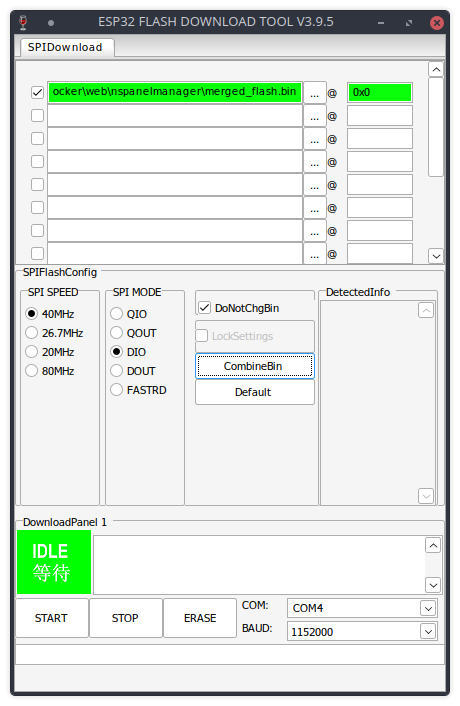
\includegraphics[scale=0.4]{esp_flash_download_tool.png}
    \end{center}
    \subsubsection{Flashing with ESPtool (all operating systems)}
    By installing esptool it is possible to upload the merged flash using the command line. Do the following:
    \begin{itemize}
      \item Open a terminal.
      \item Navigate to the "docker/web/nspanelmanager/"-directory.
      \item To determine if you have selected the right port, run \lstinline[language=bash]|esptool.py flash_id --port <port>|. You will have to replace "<port>" with the actual port connected to the NSPanel. This will do a check and see if the tool can communicate with the NSPanel.
      \item Run \lstinline[language=bash]|esptool.py --baud 921600 --port /dev/ttyUSB0 write_flash 0x0 merged_flash.bin|. You will have to replace "/dev/ttyUSB0" with the actual port connected to the NSPanel.
      \info{On Windows it might be just "esptool" without the ".py" at the end.}
      \info{On Windows "/dev/ttyUSB0" will have to be replaced by something like "COM4". If using MacOS or Linux the port will be something similar to "/dev/ttyUSB0".}
    \end{itemize}
    After the flashing is complete you can continue with \hyperref[sec:nspanel_configuration]{NSPanel configuration}.
 
    \subsection{NSPanel configuration}
    \label{sec:nspanel_configuration}
    To configure the NSPanel, do the following:
    \begin{itemize}
      \item Power up the panel.
      \warning{If you have flashed multiple NSPanels, power them up one at a time as they will all have the same WiFi access point name.}
      \info{The GUI file has not been flashed yet so there will not be any visible change on the NSPanel screen.}
      \item Connect to the new WiFi network "NSPMPanel" when the panel has started. WiFi password is \textbf{password}.
      \item When connected to the new WiFi network, make sure your device does not disconnect because it detects no internet access. Then open a browser and navigate to "http://192.168.1.1".
      \info{There have been issues when using Android and the Chrome browser that it sometimes just shows a blank page. If this is the case, either use a different browser (E.g. Firefox) or another device with WiFi to access the web page.}
      \item Enter a friendly name for the NSpanel.
      \note{This name is only used to register the NSPanel the first time. After the panel has been registered the name can be changed from the manager web interface.}
      \item Enter the IP-address for the manager docker container.
      \item Enter the port for the manager if changed during container setup.
      \item Enter WiFi name and password.
      \item Enter MQTT address and port.
      \note{If you are running the MQTT server as an add-on to Home Assistant, enter the IP-address of your Home Assistant server.}
      \item Press the "Save" button on the bottom of the page. The panel will reboot and try to connect to the WiFi network.
      \info{If the panel fails to connect to the WiFi network for three minutes it will revert back and start the access point again. It will periodically scan for the configured WiFi and, if it detetacts that the configured WiFi has come back, it will reboot and connect to it.}
      \item Connect to your WiFi again and go to the NSPanel Manager web interface. If all things are working and setup correctly the panel should show up in the list of panels on the first page.
      \info{If this is a US NSPanel version then it has to be set in the panel settings. Press the name of the NSPanel in the list and check the "Is US panel"-checkbox.}
      \item Flash the new GUI file to the panel by pressing the "Actions"-button on the right and select "Update screen".
      \note{The flashing of the GUI file may be finicky and might require multiple tries before it succeeds. If it fails and reboots or you see a "System data error", just try again.}
    \item Continue on to create new rooms and add entities to your configuration. Continue with the section on the web interface and how it work \hyperref[sec:nspanelmanager_web_interface]{here}.
    \end{itemize}

    \clearpage
    \section{NSPanel Manager web interface}
    \label{sec:nspanelmanager_web_interface}
    The web interface is partitioned into 4 main sections.
    \begin{enumerate}
      \item The first page where panel status and management can be done.
      \item The panel settings page.
      \item The Room page.
      \item The global settings.
    \end{enumerate}
    Below, each section of the web interface is described.
    \subsection{First page}
    The first page is used to get an overview of each registered NSPanel as well as perform actions on each panel. These actions are:
    \begin{itemize}
      \item Reboot.
      \item Firmware update.
      \item GUI update.
      \item Delete.
    \end{itemize}
    By pressing the name of the NSPanel you will get to the \hyperref[sec:nspanel_page]{NSPanel settings page}. Any action you want to perform on a specific panel is available as a dropdown menu from the cog. This menu includes the following options:
    \begin{itemize}
      \item \textbf{Reboot} This will send a reboot command to the NSPanel.
      \item \textbf{Visit panel page} This will open and new tab (or window) to enter the settings page on the actual NSPanel. See \hyperref[sec:nspanel_configuration]{NSPanel Configuration} for more information.
      \item \textbf{Update firmware} This will send a command to the NSPanel to start a firmware update (the update is pulled from the manager).
      \item \textbf{Update screen} This will send a command to the NSPanel to start a TFT update to the screen (the update is pulled from the manager).
      \item \textbf{Delete} Will remove the panel from this manager. The panel might still register again on next boot if the settings on the NSPanel itself are not changed.
    \end{itemize}
    There is also the "Actions"-button on the top right where you can perform some of the actions from the list above to all panels.

    \begin{figure}[H]
    \centering
    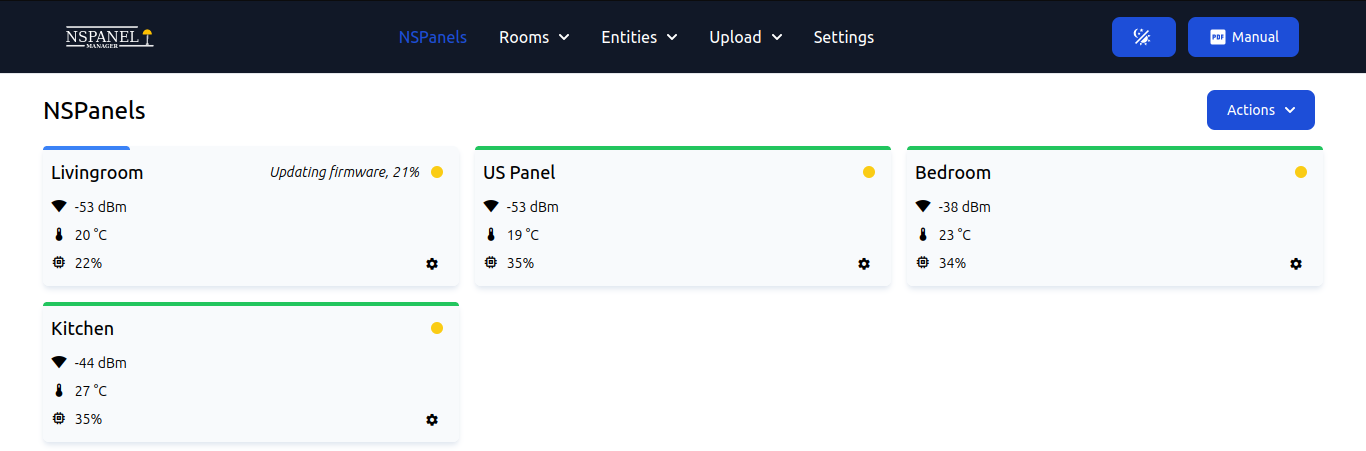
\includegraphics[width=\textwidth,height=\textheight,keepaspectratio]{index_page.png}
    \caption{Index page}%
    \end{figure}
    \subsection{NSPanel page}
    \label{sec:nspanel_page}

    On the NSPanel settings page, settings specific for one NSPanel can be made. This is things like name, default room and so on. There is also a live display of any log messages sent from the chosen NSPanel. This depends on the selected log level in the NSPanel configuration page which is available at the IP address of the NSPanel itself.

    \begin{figure}[H]
    \centering
    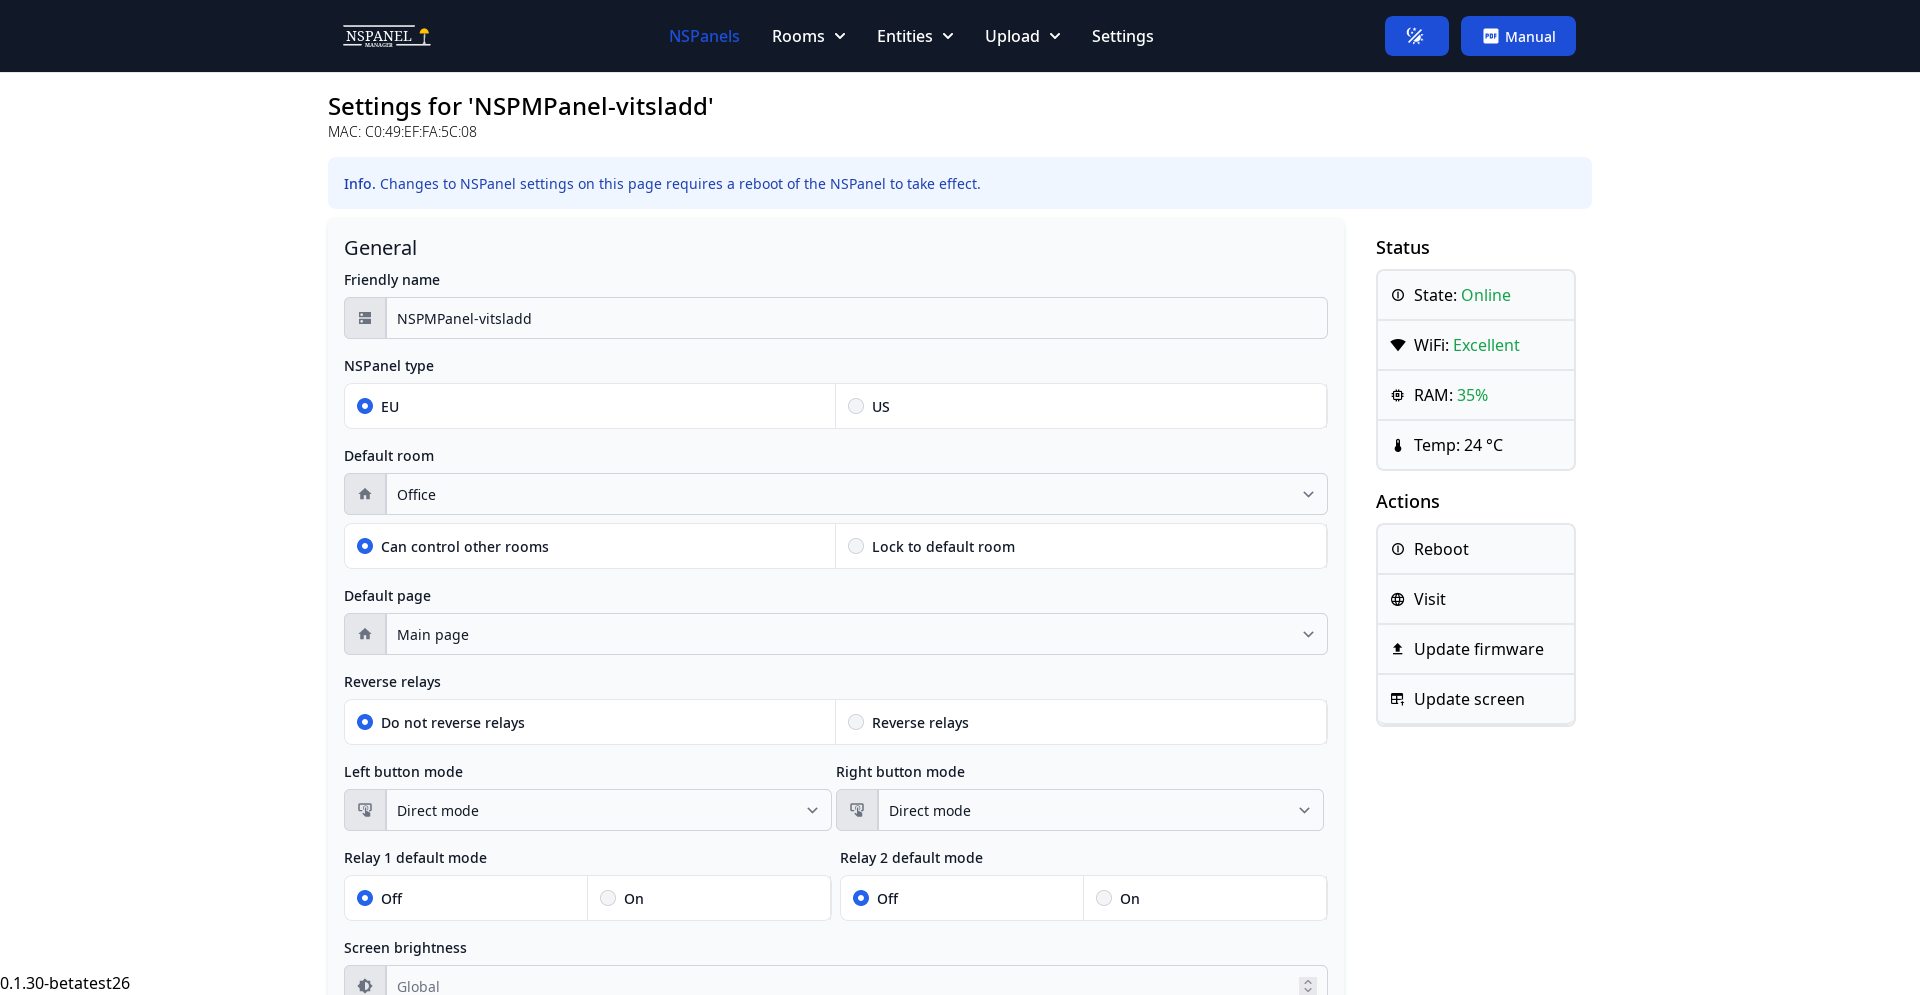
\includegraphics[scale=0.25,keepaspectratio]{nspanel_page.png}
    \caption{NSPanel page}%
    \end{figure}
    \subsection{Room page}
    \label{sec:room_page}
    
    This section will describe how to manage rooms. Most of the configuration done with NSPanel Manager will be done in rooms, please read this chapter for a full understanding on how to work with rooms.

    \begin{figure}[H]
    \centering
    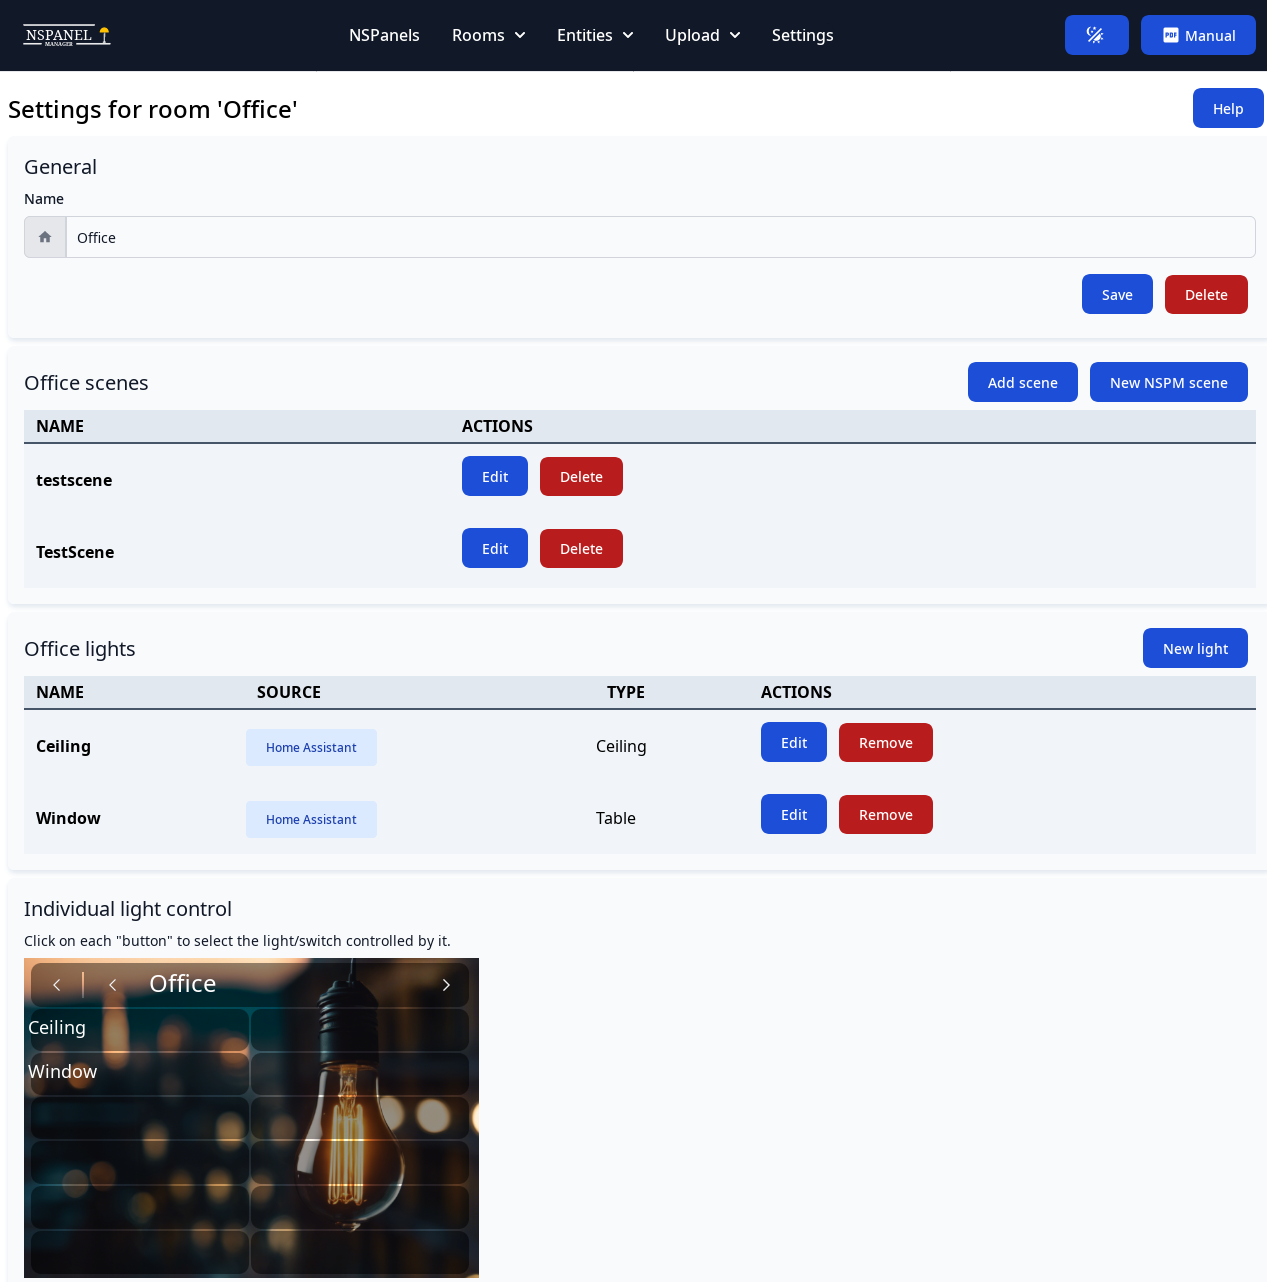
\includegraphics[width=\textwidth,height=\textheight,keepaspectratio]{room_page.png}
    \caption{Room page}%
    \end{figure}
    \subsubsection{Scenes}
    At the moment, only NSPanel Manager scenes are available. They are easy enough to use. Simply create a scenes in the room page and they will be available in the "Scenes"-list for the room on all NSPanels.
    \\ To save a scene, on the NSPanel hold the save button for the scenes for 3 seconds to save all the states of lights \textbf{currently added to the room}.
    \\ To recall/activate a scene, on the NSPanel press the name of the scene and all the saved light states will be restored for that scene.
    \note{If a light was added after a scene was saved, that light is not affected by that scenes until the scene is saved again.}
    \subsubsection{Lights}
    To add a new light, simply press the "Add new light"-button. When doing so, a list of all lights and switches gathered from Home Assistant and OpenHAB will be shown. Simply search or scroll to find the desired light and press it.
    \begin{figure}[H]
    \centering
    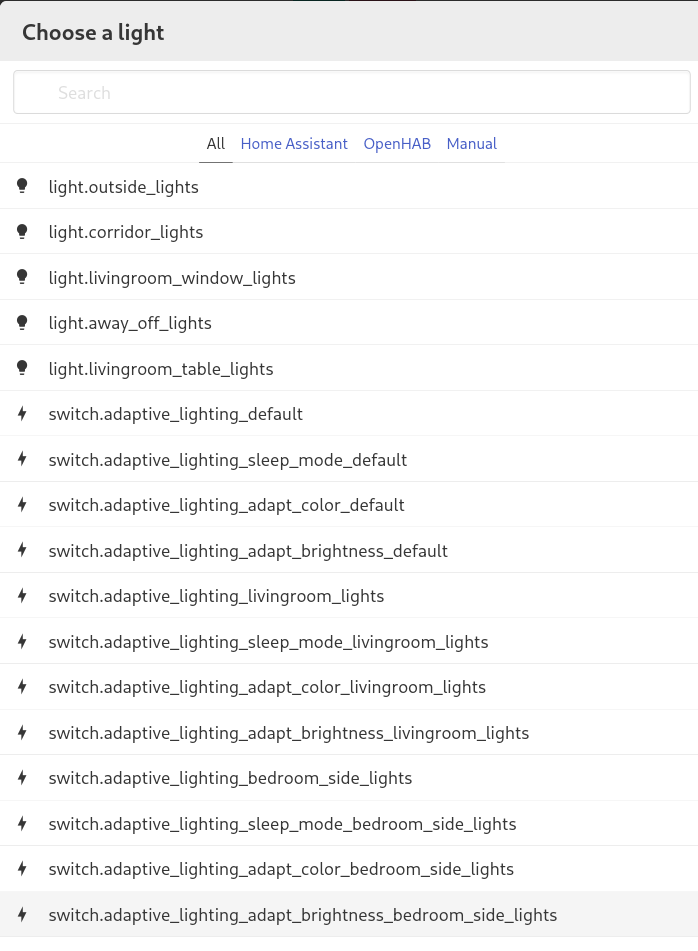
\includegraphics[scale=0.25]{add_new_light.png}
    \caption{Adding a new light to a room}%
    \end{figure}
    
    When done, a new screen will show up and depending on if the selected entity was from Home Assistant or OpenHAB.

    \begin{figure}[H]
    \centering
    \subfloat[\centering Home Assistant]{{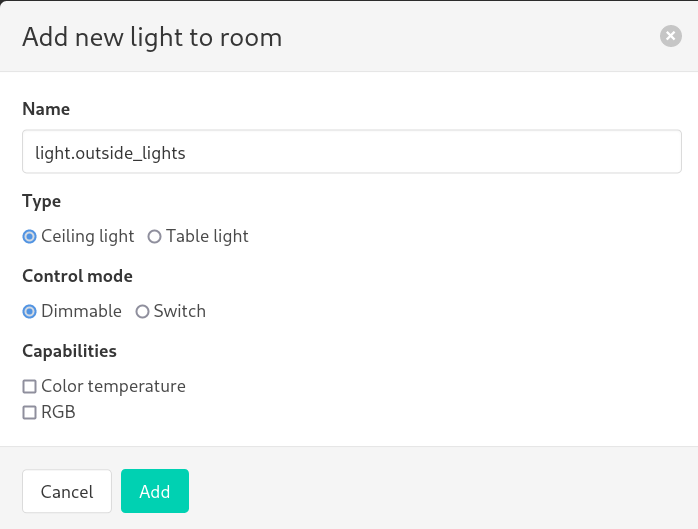
\includegraphics[width=5cm]{edit_new_light_ha.png} }}%
    \qquad
    \subfloat[\centering OpenHAB]{{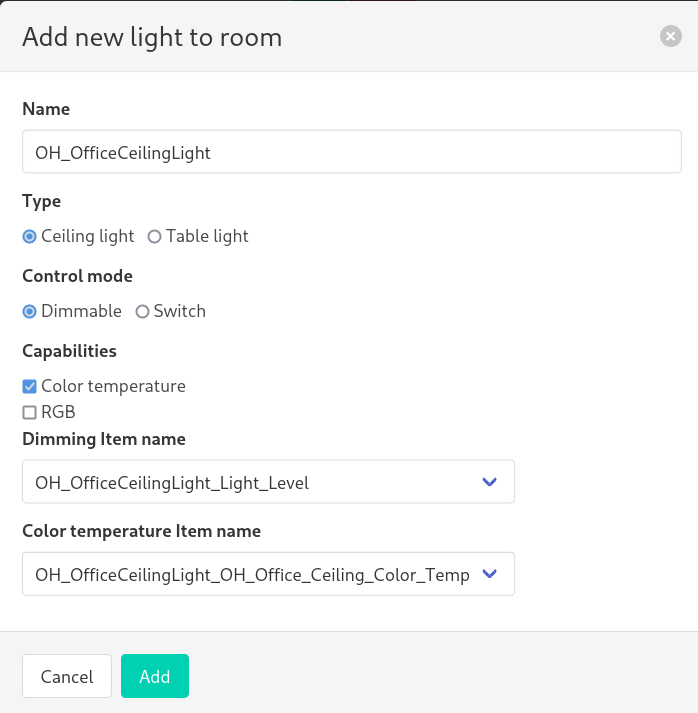
\includegraphics[width=5cm]{edit_new_light_openhab.png} }}%
    \caption{Add/Edit light}%
    \end{figure}
    
    When adding a Home Assistant entity, simply set a friendly name for it, select the type (Ceiling or Table light), select if it's a switch or dimmable light and what other capabilities it has.\\
    If you are adding an OpenHAB light or switch, things aren't as simple unfortunately. There is really no way around this but the user has to chose all the same settings as for Home Assistant but also has to select the appropriate OpenHAB items that corresponds to each capability of the light.

    \subsubsection{Individual light control}
    There is place for up to 12 lights (per room) to be controlled individually from the NSPanel. The image on the bottom shows a preview on how this might look. When a new light is added to the room it will automatically be assigned to the next free slot on the page. By pressing a slot with an assigned entity you can chose to assign a new entity (if any entity is unasigned) or "clear" the slot which will remove the light from the page but it will still be attached to the room.
    \info{Each entity may only be assigned to one slot. If the list of entities is empty then all entities has been assigned a slot.}

    \subsection{Global settings}
    These settings will apply to all NSPanels (if they do not have specific configurations), and the NSPanel Manager container. There are two things that need to be set in order to get up and running. Those are:
    \begin{enumerate}
      \item Connection details to the same MQTT server that were set in the NSPanel configuration.
      \item Connection details to Home Assistant and/or OpenHAB.
    \end{enumerate}
    \important{Failing to meet both requirements listed above will result in a non-working setup!}
    \info{If running the NSPanel Manager container as a Home Assistant add-on then the Home Assistant connection details will already be configured.}
    There are also other settings that might be worth taking a look at while here, such as global scenes that apply to all entities, showing a clock on the screensaver, how bright the NSPanels should be, the Min \& Max of color temperature and so on. Go ahead and explore by yourself.
    \begin{figure}[H]
    \centering
    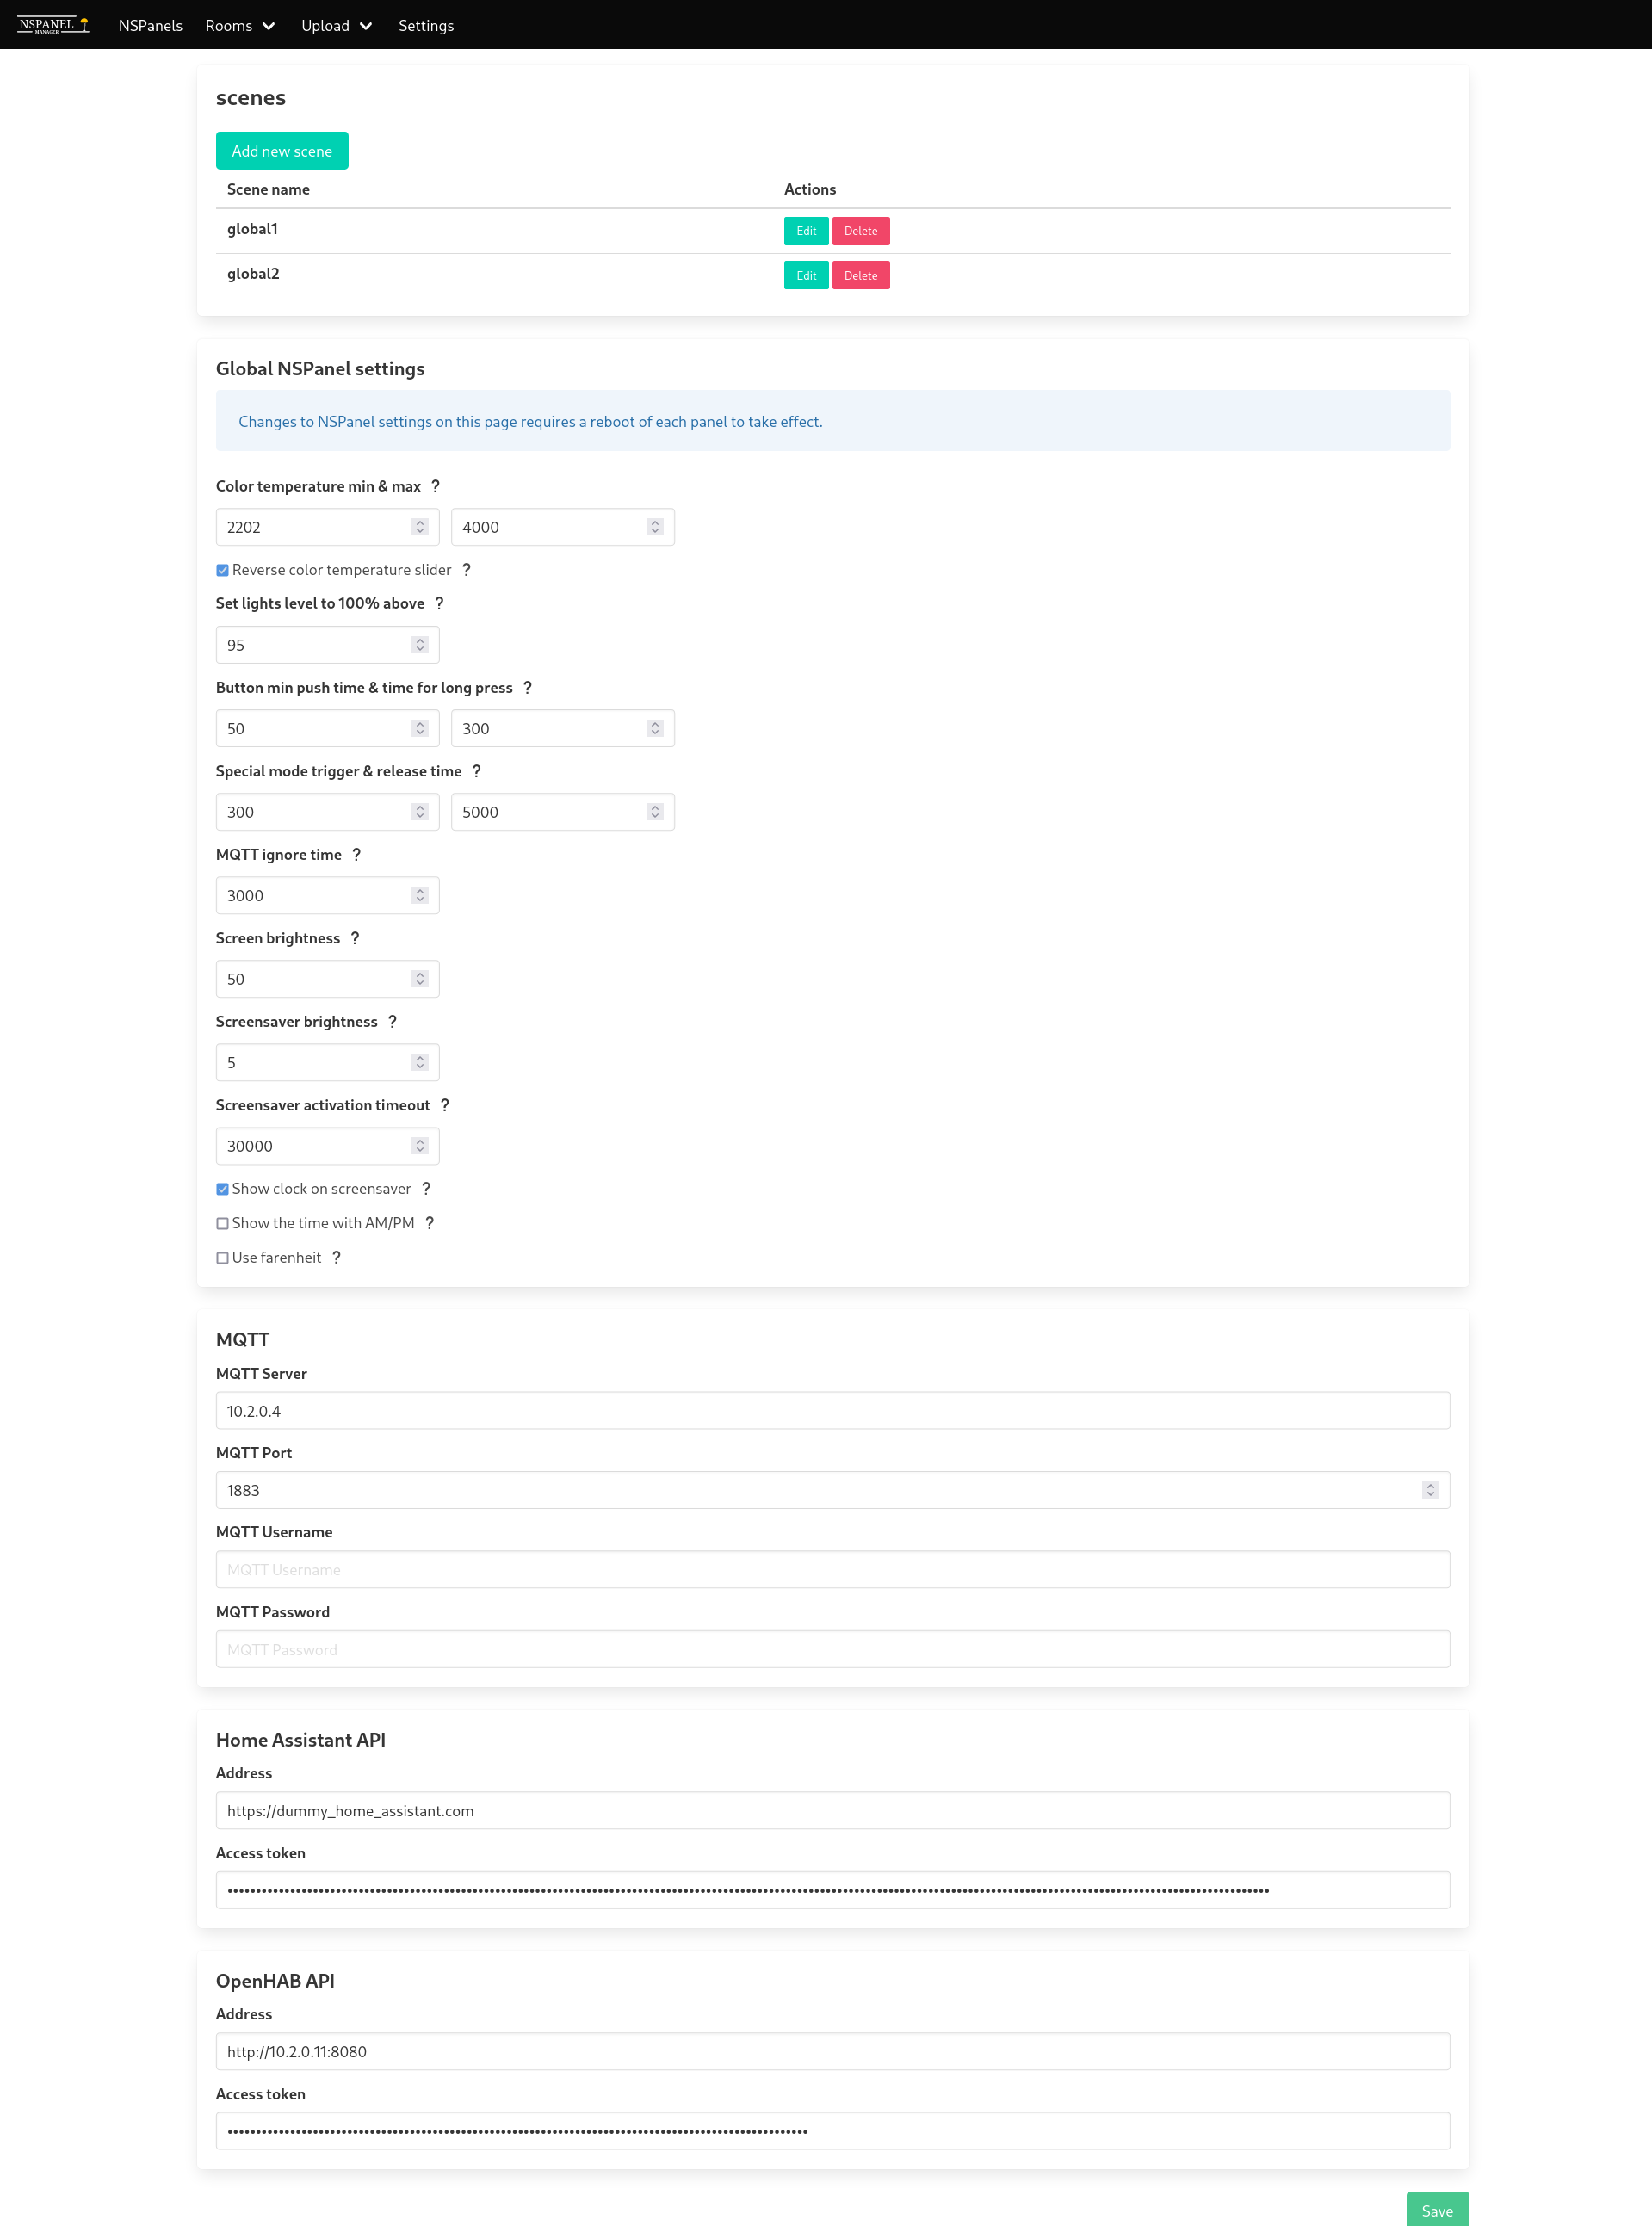
\includegraphics[scale=0.25]{settings_page.png}
    \caption{Global settings}%
    \end{figure}


    \subsection{Time and date}
    Time and date is automatically sent from the NSPanel Manager container out to each and every panel. This is used to display time and date on the screensaver (if enabled). The timezone is gathered from the TZ environment variable and automatically set.  

    \subsection{Weather}
    If you wish to use weather on the screensaver, this has to be set in the manager. In the menu bar, navigate to Entities $\rightarrow$ Weather \& Time.
    \subsubsection{Home Assistant}
    If using Home Assistant, press the "Select weather entitiy"-button and select an entity of type weather from Home Assistant.  
    Home Assistant doesn't provide sun state in the weather entity so this has to be setup manual, press the "Select sun entity"-button and select an entity of type "sun".  
    Press the save button to apply the settings.

    \subsubsection{OpenHAB}
    If using OpenHAB, there are a few things that has to be setup in OpenHAB before configuration in NSPanel Manager can happen. First of all, a weather entity for current weather has to be setup. 
    NSPanel Manager only has support for OpenWeatherMap and so, this guide will show how to setup OpenWeatherMap in OpenHAB. First of all, create an account at \href{https://home.openweathermap.org/users/sign_up}{OpenWeatherMap}.
    Once that is complete, you need to create an API-key, this can be done on \href{https://home.openweathermap.org/api_keys}{this page}. Give it a good name, something like OpenHAB so you in the future know what it's for.
    Next we will need to figure out what latitude and longitude you are located at. The easiest way of doing this is to open \href{https://maps.google.com}{Google Maps} and navigate to your location.

    Once done, the URL will look something like this:
    \begin{lstlisting}
       https://www.google.com/maps/@59.3314504,18.0823082,14.37z?entry=ttu
    \end{lstlisting}
    You latitude and longitude is placed after the @-sign, in this case the latitude is 59.3314504 and the longitude is 18.0823082.

    Next, in OpenHAB you need to install the HTTP binding from the Add-on Store. After that is done, create a new .thing-file in the "things"-directory for your OpenHAB configuration and paste the following:
    \begin{lstlisting}
    Thing http:url:weather "Weather" [
        baseURL="https://api.openweathermap.org/data/2.5/",
        refresh=600] {
            Channels:
             Type string : weather "weather" [ stateExtension="weather?units=metric&lat=<lat>&lon=<long>&appid=<apikey>" ]
             Type string : forecast "forecast" [ stateExtension="forecast?units=metric&lat=<lat>&lon=<long>&appid=<apikey>" ]
    }
    \end{lstlisting}
    \info{In case the HTTP binding does not initialize, you may need to increase the org.openhab.webclient:maxThreadsShared-value and the org.openhab.webclient:maxThreadsCustom-value in the conf/servicese/runtime.cfg-file for OpenHAB.}
    When you have pasted the above into a .things-file, you need to replace <lat> with your latitude, replace <long> with your longitude and replace <apikey> with your API-key for openweathermap.
    \info{If you do not want metric units, replace units=metric with units=imperial in the stateExtension.}
    

    \clearpage
    \section{Panel functions}
    \subsection{Main page}
    \begin{figure}[H]
    \centering
    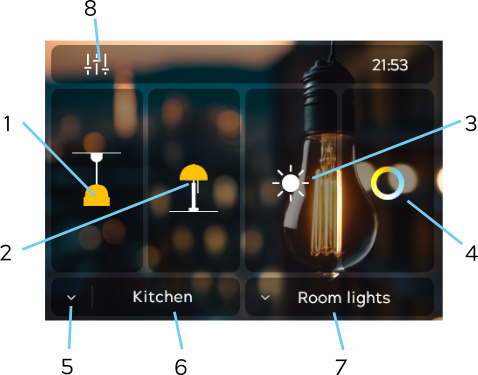
\includegraphics{main_page_numbers.png}
    \caption{Main page}%
    \end{figure}
    \bigbreak
    1. Ceiling Lights button \newline
    \textbf{Short press} - Toggle Ceiling lights ON/OFF. \newline
    \textbf{Long press} - Enter lock mode, sliders will now only effect ceiling lights. Short press to exit lock mode.
    \bigbreak
    2. Table Lights button \newline
    \textbf{Short press} - Toggle Table lights ON/OFF \newline
    \textbf{Long press} - Enter lock mode, sliders will now only effect table lights. Short press to exit lock mode.
    \bigbreak
    3. Brightness Dimmer \newline
    Control over Ceiling and Table Lights group. (More under Lights control logic below)
    \bigbreak
    4. Kelvin Dimmer \newline
    Control over Ceiling and Table Lights group. (More under Lights control logic below)
    \bigbreak
    5. Room toggle button \newline
    \textbf{Short press} - Change room.
    \bigbreak
    6. Room button \newline
    \textbf{Short press} - Enter room page for individual device control.
    \bigbreak
    7. Lights mode button \newline
    \textbf{Short press} - Toggle between Room Lights mode and All Lights mode
	  \bigbreak
    8. Scenes button. \newline
    \textbf{Short press} - Enter Scenes page. If 7 is in Room Lights mode user will enter Room Scenes. If 7 is in All Lights mode user will enter Global Scenes page.

   	\subsubsection{Lights control logic}
    The NSPanel main page might have some behavior that seems odd at first but the logic of it will be described here. The first page will affect entities in the selected room (if in room-mode) or all the configured lights (if in "All lights"-mode). The two left buttons for ceiling and table lights will always behave the same. Pressing a button that is "off" will turn on all the lights of that type. Pressing a button that is "on" will turn off all lights of that type. The sliders will always display an average value of all entities that will be affected of changes. There are few different scenarios:				

    \paragraph{One or more lights on}\mbox{} \\
    When changing the sliders, the changes will only be sent out to the lights currently on.
    If turning on a group of lights or individual lights they will be turned on to the current brightness of the slider. I.e. average dimming level in the room.
    \info{If you wish for the light to always turn on with color temperature even though you turned it off from RGB, there is a setting in the global settings.}
    
    \paragraph{No lights on}\mbox{} \\
    When changing the sliders, the changes will be sent out to all lights selected (depending on room or "all lights"-mode).
    
    \paragraph{Lock mode}\mbox{} \\
    You can lock which light to affect by pressing and holding either the ceiling or table-lights button. This will enter a special mode where changes to the sliders will only affect the selected type of lights. By pressing the same button again you can exit the "special mode". The "special mode" will also time out after a few seconds.
    
    \subsubsection{Scenes button (top left corner)}
    The little cute functional house in the top left corner is for entering the Scenes page. In NSPanel Manager there are both Room Scenes and Global Scenes. If you're in Room Lights mode (button in lower right corner) you will enter the Room Scenes page. If you're in All Lights mode you will enter the Global Scenes page. You'll also see that the house icon changes when toggling between Room Lights and All Lights mode. One yellow window and you will enter Room Scenes page when pressing it. All windows yellow and you will enter the Global Scenes page.
    \subsubsection{Swipe down}
    You can swipe downwards when on the first page to enter the Smart Home Control page.
    This page is a work in progress. Design and funcionality is not finished or decided yet.
    \subsection{Smart Home Control page}
    Accessed by swiping down on Main page. Work in progress. Design and funcionality is not finished or decided yet.  
    \subsection{Scenes page}
    To enter Scenes page, press the little house in top left corner on Main page. Depending on if you're in Room Lights mode or All Lights mode you will enter Room Scenes page or Global Scenes page.
    
    Scene names that show up here are the ones you have configured in the NSPanel Manager web interface. To store a scene simply hold the save button for three seconds and the current values of the lights in the room you are in or all lights if in All Lights mode will be saved. To activate a scene and send out those saved values you just press the scene name.
    \subsection{Room page}
	Enter Room page by pressing the room name on Main page. All devices configured for that room will show up here. To control a device individually press the device name. 
    \subsection{Individual Lights page}
    All the capabilities of the chosen light will be shown on this page. If the light is RGB capable there will be an icon in the top right corner to toggle between Color Temperature mode and Color mode.´

    \clearpage
    \section{Logs}
    \label{sec:logs}
    While logs are normally sent over MQTT, any logs that are created before WiFi-connection are sent out on Serial. If you wish to see the logs going over MQTT, you can look at the topic \lstinline[language=bash]{nspanel/<panel name>/log}. If you wish to look at the logs going over serial, you can use programs like Putty. Connect to the NSPanel with the serial programmer as usual but \textbf{dont't} connect IO0 to GND. In Putty enter your serial port in the "Serial line" box and choose baud 115200. You should then be able to connect by pressing the "Open"-button. Example:
    \info{On Windows "/dev/ttyUSB0" will have to be replaced by something like "COM4". If using MacOS or Linux the port will be something similar to "/dev/ttyUSB0".}
    \begin{figure}[H]
    \centering
    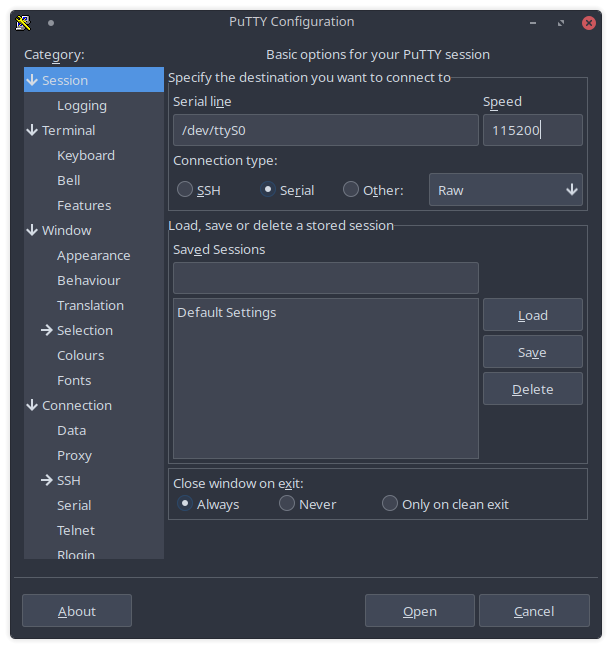
\includegraphics[scale=0.5]{putty_serial.png}
    \caption{Connecting to Serial with Putty}%
    \end{figure}

    \clearpage
    \section{Advanced setup}
    \label{sec:advanced_setup}
    \subsection{Manual Docker container setup}
    If you wish to manually build and setup the Docker container from source, use the command \\ \lstinline[language=bash]{docker build -t nspanelmanager .} while standing in the downloaded "docker"-directory. This will always be the same. To then start the container, the following command can be used:
    \note{The extra dot at the end of the "docker build"-command is essential.}
    \begin{lstlisting}[language=bash]
    docker run --name nspanelmanager -v /etc/timezone:/etc/timezone:ro -v \
    "$(pwd)/data/":"/data/" \
    -d -p 8000:8000 -p 8001:8001 nspanelmanager
    \end{lstlisting}
    If you wish to change the timezone, there are two options. Either, do as the command above, pass in the local machine /etc/timezone. This might not always work though as your server might be set to Etc/UTC then you can set the TZ-environment variable, for example: \lstinline[language=bash]{-e TZ=Europe/Stockholm} and remove the volume mapping for /etc/timezone.
    \important{All data for NSPanel Manager is stored in the directory mapped to "/data" in the container. In this case, the "data"-directory where you are currently standing.}


    \subsection{Docker-compose container setup}
    If you wish to run NSPanel manager from docker compose you can use the below example as a template for your setup.
    \note{This example is for an x86\_64 machine placed in the Europe/Stockholm timezone. Replace image name and timezone as needed.}
    \begin{lstlisting}
    services:
      nspanelmanager:
        image: nspanelmanager/nspanelmanager-amd64
        container_name: nspanelmanager
        environment:
          - TZ=Europe/Stockholm
        volumes:
          - /nspmdata/:/data/
        ports:
          - 8000:8000
          - 8001:8001
        restart: always
    \end{lstlisting}
    \important{All data for NSPanel Manager is stored in the directory mapped to "/data" in the container. In this case, the "/nspmdata/"-directory where you are currently standing.}

    \clearpage
    \section{Functional information}
    \subsection{Software components}
    There are really three software components written for the NSPanel Manager project. These are described as below:
    \begin{itemize}
      \item \textbf{Web interface:} The web interface that you interact with is built on top of the Django framework. This software gives the user an interface to interact and configure the project with. This software also manages the database with settings.
      \item \textbf{MQTT Manager:} There is a second software running in the background on the NSPanel Manager container that hosts the web interface. This component is named "MQTTManager". The MQTTManager handles all things with MQTT. It loads the config from the web interface via the API and then processes all commands from panels, state updates from Home Assistant and OpenHAB and so on. It's basically the glue that makes the panel's actions affect Home Assistant and OpenHAB. The MQTTManager is also the software that send state updates from Home Assistant and OpenHAB to the panels when changes occur.
      \item \textbf{The NSPanel firmware:} The firmware written for the NSPanel has been specifically designed to be as response and easy to use as possible. The firmware handles all communication with the TFT (Nextion) display and with MQTTManager via MQTT.
    \end{itemize}

    \subsection{Data flow}

    \begin{figure}[H]
    \centering
    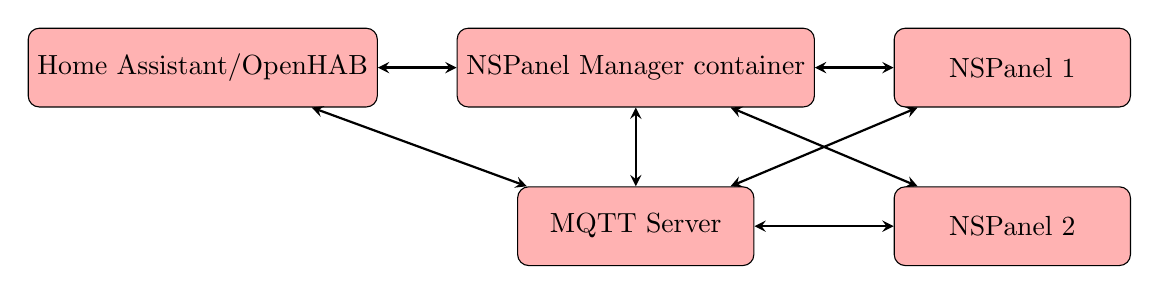
\begin{tikzpicture}
      \node (HAOpenHab) [startstop] {Home Assistant/OpenHAB};
      \node (NSPMcontainer) [startstop, right=of HAOpenHab] {NSPanel Manager container};
      \draw [doublearrow] (HAOpenHab) -- (NSPMcontainer);
      \node (MQTT) [startstop, below=of NSPMcontainer] {MQTT Server};
      \draw [doublearrow] (HAOpenHab) -- (MQTT);
      \draw [doublearrow] (NSPMcontainer) -- (MQTT);

      \node (panel1) [startstop, right=of NSPMcontainer] {NSPanel 1};
      \node (panel2) [startstop, below=of panel1] {NSPanel 2};
      \draw [doublearrow] (NSPMcontainer) -- (panel1);
      \draw [doublearrow] (NSPMcontainer) -- (panel2);
      \draw [doublearrow] (MQTT) -- (panel1);
      \draw [doublearrow] (MQTT) -- (panel2);
    \end{tikzpicture}
    \caption{NSPanel Manager data flow}%
    \end{figure}

    The data flow within NSPanel Manager might look intimidating but it's not that bad. Below is an explanation of all the arrows above.

    
    \subsubsection{Home Assistant and/or OpenHAB to/from NSPanel Manager container}
    There is two types of traffic flowing between these nodes:
    \begin{itemize}
      \item \textbf{Websocket:} A websocket connection is setup in order for the NSPanel Manager container to receive entity updates from Home Assistant and/or OpenHAB but also to sent entity commands (E.. turn light X on to 20\%). A websocket is used to speed up the communication and also to not have to poll the home automation software for information.
      \item \textbf{HTTP GET API:} The usual HTTP GET API is also used. This is used when adding entities to a room, as an example. When pressing the "Add new light" button, the NSPanel Manager container will make an HTTP GET request to gather all available entities and then send them back to the client (browser) so that the user may choose what entitiy to add to the room.
    \end{itemize}
    \subsubsection{NSPanel Manager container to/from MQTT}
    MQTT is used to send updated entity states received from the home automation software out to all NSPanels and also receive states and commands from NSPanels.
    \subsubsection{Home Assistant and/or OpenHAB to/from MQTT}
    Home Assistant and OpenHAB can leverage the MQTT integration through "Home Assistant MQTT Auto-discovery" (which OpenHAB can also use) to auto-discover NSPanels and automatically register entities for panel temperature reading, panel relays, screen state and so on.
    \subsubsection{NSPanel Manager container to/from NSPanels}
    The configuration of lights, scenes and so on does not reside on each panel. The panel only has localy the bare minimum configuration for setup. When the panel starts and has connected to WiFi it will do a HTTP GET request to the NSPanel Manager container in order to receive all configuration of entities, screen brightness and really, all settings available in the NSPanel Manager web interface.
    \subsubsection{MQTT to/from NSPanels}
    Each NSPanel send states (E.g. temperature) and commands (E.g. turning on a light) over MQTT for the NSPanel Manager container to pickup. The panel also received commands, E.g. turn on relay 1, turn on screen and so on.

    \subsection{MQTT Topics}
    Below table is a description of all MQTT topics that might be of use by a user. Replace <panel\_name> with the friendly name of your NSPanel:
    \begin{table}[H]
    \begin{tabular}{|l|l|l|}
    \hline
    \textbf{Topic} & \textbf{Payload}  & \textbf{Description}  \\ \hline
    nspanel/<panel\_name>/screen\_cmd & 1 or 0 & Send a 1 or 0 to turn on/off the display. \\ \hline
    nspanel/<panel\_name>/screen\_state & 1 or 0 & Current state of the screen. \\ \hline
    nspanel/<panel\_name>/brightness & 1 to  100 & Control the brightness of the screen. \\ \hline
    nspanel/<panel\_name>/brightness\_screensaver & 0 to  100 & Control the brightness of the screensaver. \\ \hline
    nspanel/<panel\_name>/r1\_cmd & 1 or 0 & Send a 1 or 0 to turn on/off relay 1. \\ \hline
    nspanel/<panel\_name>/r1\_state & 1 or 0 & The current state of relay 1. \\ \hline
    nspanel/<panel\_name>/r2\_cmd & 1 or 0 & Send a 1 or 0 to turn on/off relay 2. \\ \hline
    nspanel/<panel\_name>/r2\_state & 1 or 0 & The current state of relay 2. \\ \hline
    nspanel/<panel\_name>/temperature\_state & Current temperature & The current temperature reading. \\ \hline
    nspanel/<panel\_name>/log & Log message & The panel will send live logs on this topic. \\ \hline
    \end{tabular}
    \end{table}

    There are more topics that are used internally, these are:

    \begin{table}[H]
    \centering
    \resizebox{\textwidth}{!}{\begin{tabular}{|l|l|L{8cm}|}
    \hline
    \textbf{Topic} & \textbf{Payload}  & \textbf{Description}  \\ \hline
    nspanel/entities/<type>/<id>/state\_<attribute> & The value of the attribute & An update of entity state value sent out by MQTTManager. Example: nspanel/entities/light/42/state\_kelvin \\ \hline
    nspanel/status/time & Time & Current time sent by MQTTManager. \\ \hline
    nspanel/<panel\_name>/status\_report & JSON & JSON payload with current state of the panel. \\ \hline
    nspanel/mqttmanager/command & JSON & JSON payload from panel with a command for MQTTManager to perform. \\ \hline
    \end{tabular}}
    \end{table}


\end{document} % This is the end of the document
